\chapter{Supplementary Material}

% Reset figure and table counters and change format
\setcounter{figure}{0}
\setcounter{table}{0}
\renewcommand{\thefigure}{S\arabic{figure}}
\renewcommand{\thetable}{S\arabic{table}}

\section*{Supplementary Figures}

\begin{figure}[H]
  \centering
  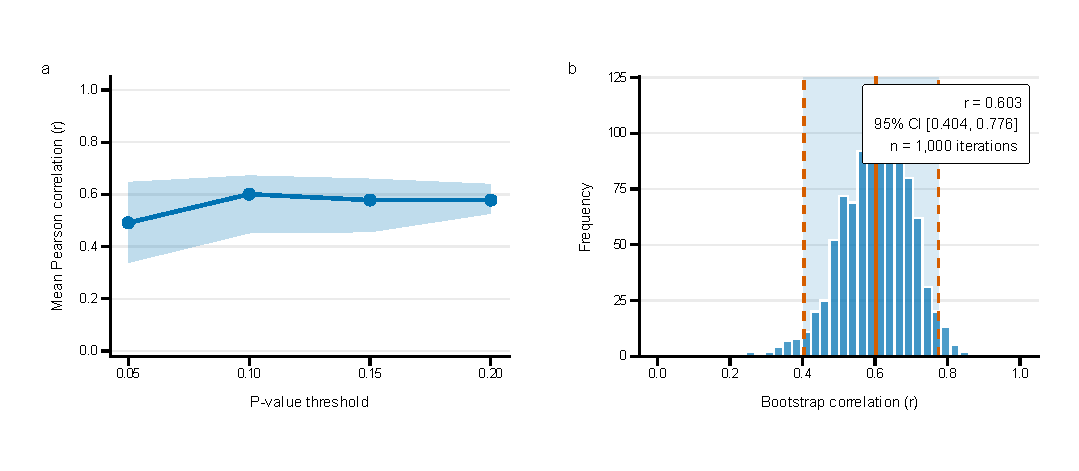
\includegraphics[width=\textwidth]{../../paper/figures/output/pdf/figS1_cross_species_sensitivity.pdf}
  \caption{\textbf{Cross-species sensitivity analysis of conserved developmental markers.}
  \textbf{a}, Mean Pearson correlation between pig and human developmental fold changes across significance thresholds ranging from $p < 0.01$ to $p < 0.20$. Shaded region indicates the range (minimum--maximum) across different gene set sizes ($n = 15$--$50$ genes).
  \textbf{b}, Bootstrap distribution of correlation coefficients ($n = 1{,}000$ iterations) for the optimal parameter combination ($p < 0.10$, $n = 36$ genes). Solid vertical line indicates the observed correlation ($r = 0.603$); dashed lines denote the 95\% bootstrap confidence interval boundaries (0.404--0.776).}
  \label{fig:S1}
\end{figure}

\clearpage

\begin{figure}[H]
  \centering
  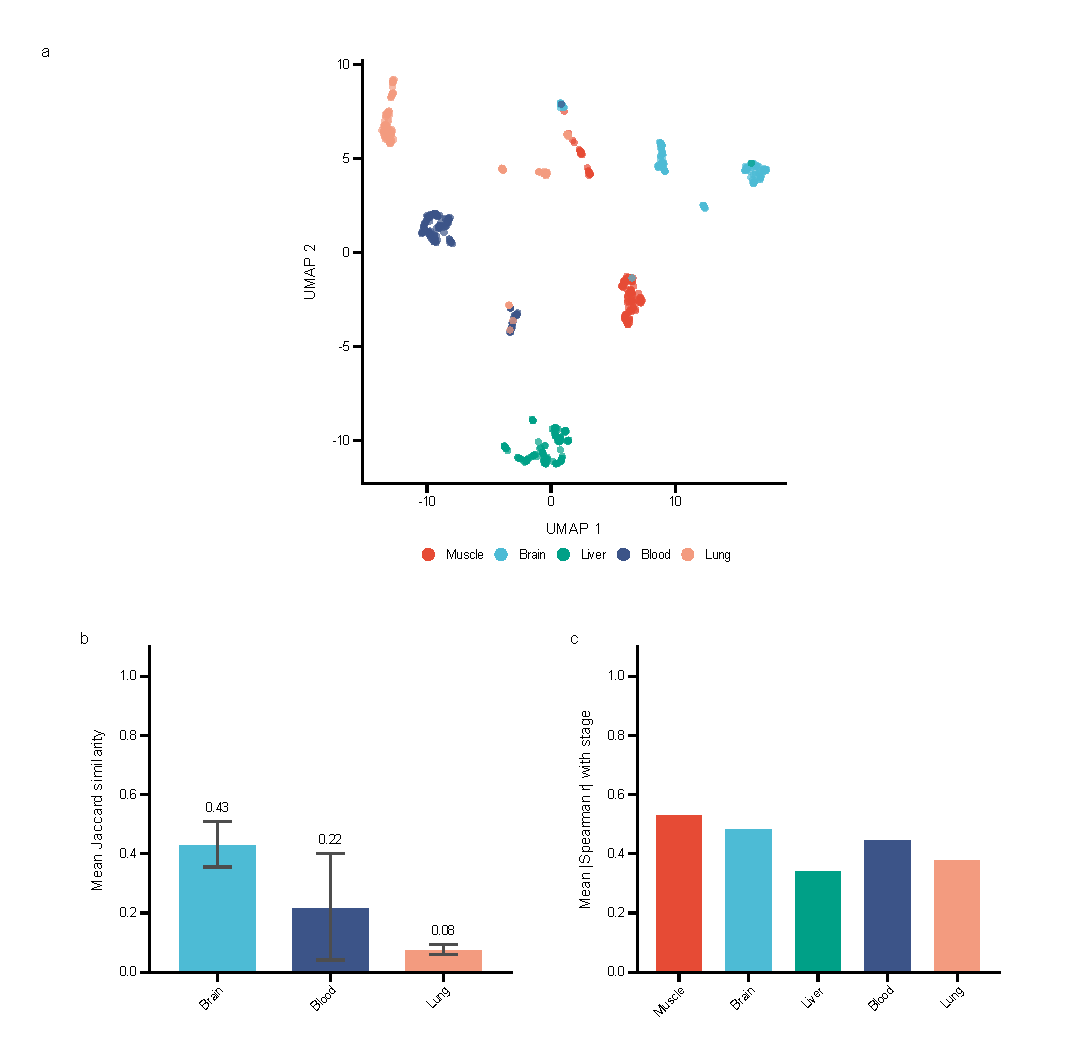
\includegraphics[width=\textwidth]{../../paper/figures/output/pdf/figS2_tissue_specificity_stability.pdf}
  \caption{\textbf{Tissue specificity and feature selection stability analysis.}
  \textbf{a}, Uniform manifold approximation and projection (UMAP) \parencite{mcinnes_umap_2018} of gene expression profiles across five tissues (muscle, brain, liver, blood, lung), demonstrating distinct tissue-specific clustering patterns ($n = 150$ samples per tissue, balanced sampling; top 500 variable genes).
  \textbf{b}, Within-tissue feature selection stability quantified as mean Jaccard similarity index of the top 50 selected features across five independent random seeds (brain, blood, lung; stability analysis not performed for muscle and liver). Error bars represent standard deviation; higher values indicate more reproducible feature selection.
  \textbf{c}, Mean absolute Spearman correlation between top-ranked features and developmental stage for each tissue.}
  \label{fig:S2}
\end{figure}

\clearpage

\begin{figure}[H]
  \centering
  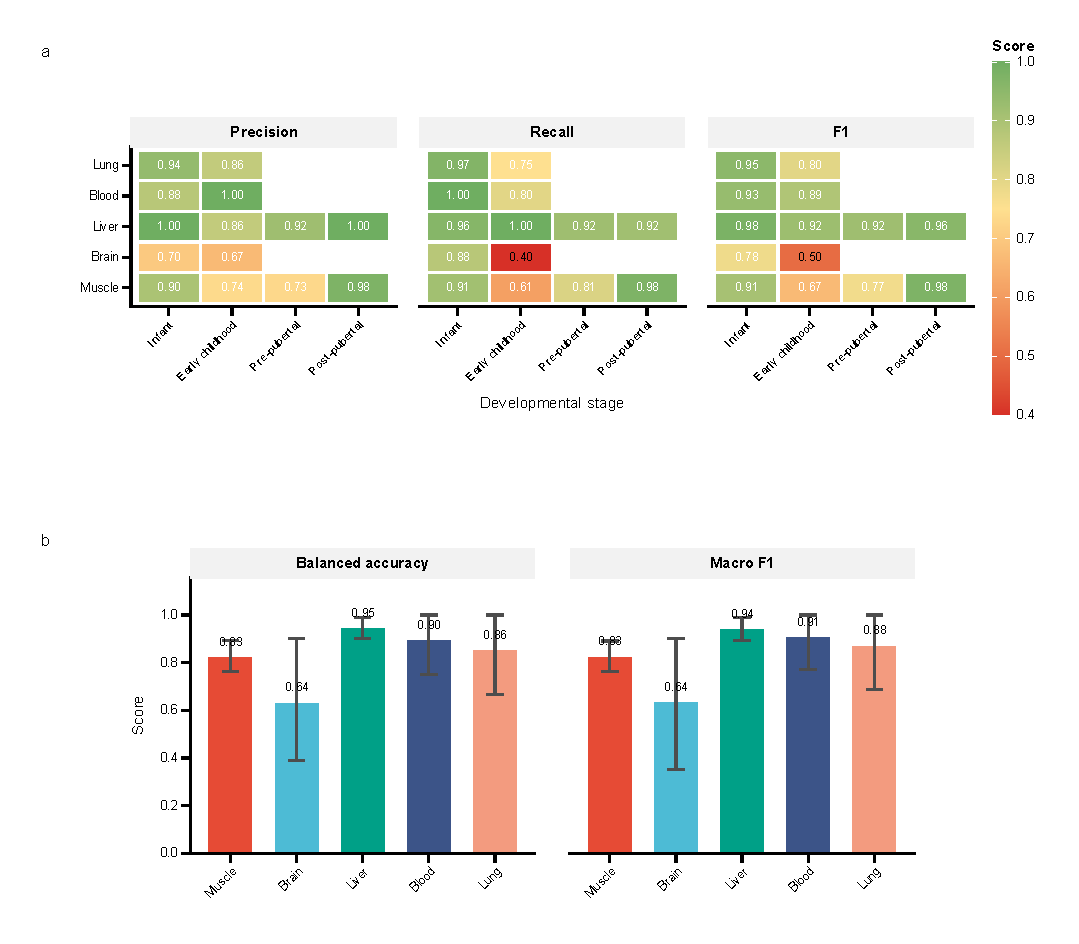
\includegraphics[width=\textwidth]{../../paper/figures/output/pdf/figS3_extended_performance.pdf}
  \caption{\textbf{Extended classification performance metrics across tissues and developmental stages.}
  \textbf{a}, Heatmap of per-class precision, recall, and F1 scores for each developmental stage across all five tissues. Colour scale ranges from 0.4 (red, poor performance) to 1.0 (green, excellent performance). Missing values indicate developmental stages not present in that tissue's classification scheme.
  \textbf{b}, Overall performance summary showing balanced accuracy and macro-averaged F1 scores evaluated on the held-out test set (30\% of samples) for each tissue. Error bars indicate 95\% bootstrap confidence intervals from 1,000 resampling iterations.}
  \label{fig:S3}
\end{figure}

\clearpage

\section*{Supplementary Tables}

\begin{table}[H]
  \centering
  \caption{\textbf{Train versus test performance comparison.} Test set performance (30\% held out) is reported for all tissues. Train set metrics are not shown as models were evaluated only on held-out data to prevent overfitting.}
  \label{tab:S1}
  \small
  \begin{adjustbox}{max width=\textwidth}
  \begin{tabular}{lcccccc}
    \toprule
    Tissue & Scheme & $n$ & Balanced Acc. & F1-macro & F1-weighted & MAE \\
    \midrule
    Muscle & 4-class & 761 & 0.844 & 0.842 & 0.908 & 0.10 \\
    Brain & 2-class & 43 & 0.637 & 0.639 & 0.671 & -- \\
    Liver & 4-class & 309 & 0.920 & 0.910 & 0.913 & 0.09 \\
    Blood & 2-class & 78 & 0.864 & 0.869 & 0.874 & -- \\
    Lung & 2-class & 129 & 0.859 & 0.876 & 0.921 & -- \\
    \bottomrule
  \end{tabular}
  \end{adjustbox}

\end{table}

\vspace{1cm}

\begin{table}[H]
  \centering
  \caption{\textbf{Per-class performance metrics by tissue.} Precision, recall, and F1 scores for each developmental stage within each tissue. $n$ indicates the number of test samples per class.}
  \label{tab:S2}
  \small
  \begin{adjustbox}{max width=\textwidth}
  \begin{tabular}{llcccc}
    \toprule
    Tissue & Stage & $n$ & Precision & Recall & F1 \\
    \midrule
    Muscle & Infant & 58 & 0.912 & 0.897 & 0.904 \\
    Muscle & Early childhood & 23 & 0.714 & 0.652 & 0.682 \\
    Muscle & Pre-pubertal & 27 & 0.767 & 0.852 & 0.807 \\
    Muscle & Post-pubertal & 121 & 0.975 & 0.975 & 0.975 \\
    \midrule
    Brain & Infant & 8 & 0.700 & 0.875 & 0.778 \\
    Brain & Early childhood & 5 & 0.667 & 0.400 & 0.500 \\
    \midrule
    Liver & Infant & 26 & 1.000 & 0.962 & 0.980 \\
    Liver & Early childhood & 18 & 0.783 & 1.000 & 0.878 \\
    Liver & Pre-pubertal & 25 & 0.950 & 0.760 & 0.844 \\
    Liver & Post-pubertal & 24 & 0.920 & 0.958 & 0.939 \\
    \midrule
    Blood & Infant & 14 & 0.867 & 0.929 & 0.897 \\
    Blood & Early childhood & 10 & 0.889 & 0.800 & 0.842 \\
    \midrule
    Lung & Infant & 31 & 0.938 & 0.968 & 0.952 \\
    Lung & Early childhood & 8 & 0.857 & 0.750 & 0.800 \\
    \bottomrule
  \end{tabular}
  \end{adjustbox}

\end{table}

\clearpage

\begin{table}[H]
  \centering
  \caption{\textbf{Functional annotations of key developmental markers.} Annotations compiled from UniProt, GeneCards, and literature review. All listed genes show conserved developmental expression patterns between pig and human muscle tissue. FC = log$_2$ fold change (infant vs.\ adult). Pig FC derived from pig GTEx data (GEO: GSE257558); Human FC from \textcite{schaiter_molecular_2024}.}
  \label{tab:S3}
  \footnotesize
  \singlespacing
  \begin{tabularx}{\textwidth}{lXcc}
    \toprule
    Gene & Developmental Function & Pig FC & Human FC \\
    \midrule
    \textit{SORCS2} & Serves as a molecular switch directing trafficking of key signalling receptors to regulate the balance between neuronal growth and pruning, ensuring precise wiring of the developing nervous system \parencite{thomasen_sorcs2_2023}. & 1.84 & 0.95 \\
    \addlinespace
    \textit{FGFRL1} & Acts as a ``decoy'' receptor dampening excessive growth factor signalling to ensure proper formation of critical structures including the diaphragm, kidneys, and skeleton \parencite{amann_fgfrl1_2014}. & 1.68 & 2.10 \\
    \addlinespace
    \textit{KREMEN1} & Functions as a critical negative regulator of Wnt signalling, partnering with Dkk1 to control cell survival and ensure proper patterning of organs including thymus, teeth, and neural tissues \parencite{osada_wnt_2006}. & 1.25 & 1.43 \\
    \addlinespace
    \textit{ACHE} & Functions not only as an enzyme regulating chemical signalling to prevent cell damage but also as a structural adhesion molecule guiding physical growth of neurons and brain wiring \parencite{rotundo_expression_2003}. & 1.81 & 0.53 \\
    \addlinespace
    \textit{MSS51} & Acts as a skeletal muscle-specific ``brake'' on metabolism, regulating mitochondrial respiration and energy expenditure as muscle fibres differentiate and mature \parencite{rovira_gonzalez_mss51_nodate}. & $-$3.02 & $-$1.55 \\
    \addlinespace
    \textit{IGSF1} & Regulates the neuroendocrine system by modulating signal transduction in the pituitary gland, enabling maturation of the thyroid axis and coordination of testicular development \parencite{joustra_igsf1_2019}. & 2.45 & 0.34 \\
    \addlinespace
    \textit{PDLIM3} & Acts as a cytoskeletal scaffolding protein stabilising actin filaments at the muscle Z-disc, playing a critical role in ensuring structural integrity of the heart \parencite{ohsawa_alternative_2011}. & $-$2.19 & $-$0.56 \\
    \bottomrule
  \end{tabularx}
\end{table}
